\documentclass[a4paper, 12pt]{article}

\usepackage{graphicx}
\usepackage{xcolor}
\usepackage{mdframed}
\usepackage { amsmath , amssymb , amsthm }
\usepackage[T2A]{fontenc}
\usepackage[utf8]{inputenc}
\usepackage[english,russian]{babel}

\graphicspath{{img/}}
\DeclareGraphicsExtensions{.pdf,.png,.jpg}


\title{Инженерная графика}
\author{Щербинин В.В}
\date{\today}

\begin{document}
\sffamily
\maketitle

\section*{Введение}

ЕСКД -- единая система конструкторской документации (устанавливает взаимосвязь правил по оформлению, конструированию, обращинию конструкторской документации)\\
"+":\\
1. Возможность взаимообмена конструкторской документации между предприятиями.\\
2. Стабилизация комплектности, исключающая дубрированость документов.\\
3. Возможность обеспечивать унификации при конструировании, разработке, проэктированиии комерческих изделий\\
4. Упращенная форма конструкторской документации.\\
5. Механизм и автоматизм обработки технической документации.\\
\newpage
\section{Методы проекции}

\subsection{Центральная проекция}
Для получения центральных проекций необходимо задаться плоскостью проекций H и центром проекций S.\\
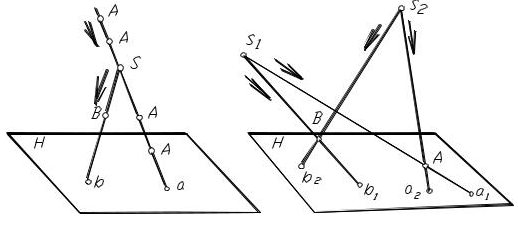
\includegraphics{eng1}\\
Центр проекций действует как точечный источник света, испуская проецирующие лучи. Точки пересечения проецирующих лучей с плоскостью проекций H называются проекциями. Проекций не получается, когда центр проецирования лежит в данной плоскости или проецирующие лучи параллельны плоскости проекций.\\

Свойства центрального проецирования:\\
1.Каждая точка пространства проецируется на данную плоскость проекций в единственную проекцию.\\
2.В то же время каждая точка на плоскости проекций может быть проекцией множества точек, если они находятся на одном проецирующем луче\\
3.Прямая, не проходящая через центр проецирования, проецируется прямой (проецирующая прямая – точкой).\\
4.Плоская (двумерная) фигура, не принадлежащая проецирующей плоскости, проецируется двумерной фигурой (фигуры, принадлежащие проецирующей плоскости, проецируются вместе с ней в виде прямой).\\
5.Трехмерная фигура отображается двумерной.\\
Глаз, фотоаппарат являются примерами этой системы изображения. Одна центральная проекция точки не дает возможность судить о положении самой Точки в пространстве, и поэтому в техническом черчении это проецированиепочти не применяется. Для определения положения точки при данном способе необходимо иметь две ее центральные проекции, полученные из двух различных центров. Центральные проекции применяют для изображения предметов в перспективе. Изображения в центральных проекциях наглядны, но для технического черчения неудобны.

\subsection{Параллельная проекция и их свойства}
Параллельное проецирование – частный случай центрального проецирования, когда центр проецирования перемещен в несобственную точку, т.е. в бесконечность. При таком положении центра проекций все проецирующие прямые будут параллельны между собой. В связи с параллельностью проецирующих прямых рассматриваемый способ называется параллельным, а полученные с его помощью проекции – параллельными проекциями. Аппарат параллельного проецирования полностью определяется положением плоскости проецирования (H) и направлением проецирования.\\

Свойства параллельного проецирования:\\
1.При параллельном проецировании сохраняются все свойства центрального проецирования, а также возникают новые:\\
2.Для определения положения точки в пространстве необходимо иметь две ее параллельные проекции, полученные при двух различных направлениях проецирования.\\
3.Параллельные проекции взаимно параллельных прямых параллельны, а отношение длин отрезков таких прямых равно отношению длин их проекций.\\
4.Если длина отрезка прямой делится точкой в каком-либо отношении, то и длина проекции отрезка делится проекцией этой точки в том же отношении .\\
5.Плоская фигура, параллельная плоскости проекций , проецируется при параллельном проецировании на эту плоскость в такую же фигуру.\\

Параллельное проецирование, как и центральное, при одном центре проецирования, также не обеспечивает обратимости чертежа.\\
Применяя приемы параллельного проецирования точки и линии, можно строить параллельные проекции поверхности и тела.\\

\subsection{Прямоугольное (ортогональное)проецирование}

\textbf{Прямоугольное проецирование} -- это частный случай параллельного проец при котором проецирующие прямые перпендикулярны плоскости проекции и параллельны друг-другу.
\\
Ортогональные проекции двух взаимно перпендикулярных прямых, одна из которых параллельны плоскоти проекций а другая не перпендикулярна ей взаимно перпендикулярны.\\
Преймущества:\\
1. простота\\
2. при ортогональном проецировании, при ряди условий удается сохранить форму и размеры фигуры.\\

\subsection{Проецирование на две взаимно перпендикулярные плоскости проекции}
Обратимость чертежа может быть обеспечена проецированием на две плоскости проекции.\\

Состоит из фронтальной и горезонтальной плоскастей проекций, а линия пересечения называется осью проекции и называбт x или v/h.\\
%вставить рисунок взаимно перпендикулярных плоскостей

В некоторых случаях удобней использовать\\
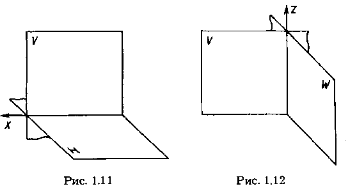
\includegraphics{143}\\
состоит из фронтальной и профильной плоскотей проекций, ось пересечения называется v/w.\\

Горизонтальные проекции точки называют прямоугольную проекцию точки на горизонтальную плоскость проекции.\\
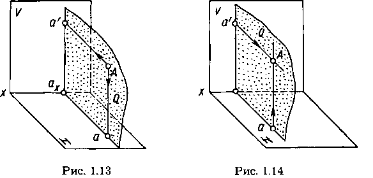
\includegraphics{eng141}\\
%вставить рисунок проецирования v/h
обозначения: $ a $ на h , $ a' $ на v для точки $ A $\\
плоскость Q перпендикулярна плоскостям проекции и пересекает ось проекции x\\
Для того чтобы востановить положение A необходимо востановить перпендикуляры к плоскостям проекций в $a \quad a'$, на пересечении перпендикуляров находится точка A\\
Две параллельные проекции точки на различные плоскости проекции вполне определяют ее положение в пространстве, а значит проецирование на две ортогональных плоскости проекции обеспечивает обратимость чертежа для точки.\\

Эпюры Моджа:\\
%рисунок
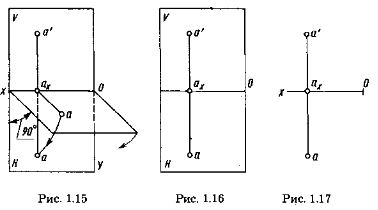
\includegraphics{142}\\
Отрезок a'a называетс линией связи\\

\subsection{Проецирование на три взаимно перпендикулярные плоскости проекции}

%рисунок трех плоскостей проекции
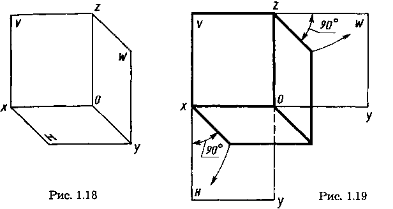
\includegraphics{151}
называется V,H,W. Точка O - пересечение трех проекций.\\

Принято разрезать ось y\\

!!!Помнить про чертову прямую -45 градусов\\
При параллельных прямых все их проекции параллельны!!!\\

\section{Глава. Проецирование отрезка прямой линии}
\subsection{Проецирование отрезка прямой линии и деление его в заданном отношении}

Отрезки $a_p \quad b_p$ ледат в некоторой плоскости Q, эта плоскость перпендикулярна плоскости P, прямая, по которой плоскость Q пересекает плоскость P содержит точки AB\\
\begin{center}
	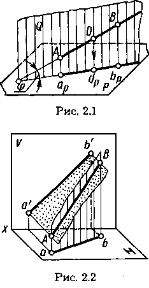
\includegraphics{img/211.png}
\end{center}


если точка принадлежит никакому отношению то ее проекции принадлежат одноименным проекциям отрезка и делят их в одном и томже отношении.
\\

\subsection{Положение прямой линии относительно плоскостей проекции. Особые случаи положения прямой}
1. прямая не параллельна ни одной из плоскостей проекции(прямая общего положения)\\
2. прямая параллельны одной из плоскостей проекции или ей принадлежит(прямая частного положения)\\
3. параллельна двум плоскостям проекции и перпендикулярна третей(прямая частного положения)\\
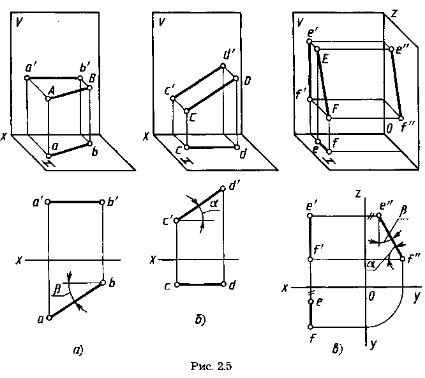
\includegraphics{img/221.png}\\
Соответственно называется фронтальной или профильной прямой(в зависимости какой параллельна плоскости).\\
Если прямая перпендикулярна одной из плоскостей проекции то она называется проецирующей для этой плоскости(горизонтально,фронтально,профильно проецирующией)\\
Проецирующая прямая проецируется на соответствующиую плоскость проекции в точку.\\

\subsection{Определение натуральной велечины прямой, общего положения и углов его наклона к плоскостям проекции}
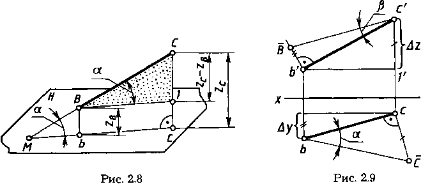
\includegraphics{img/231.png}\\
Итак, натуральную величину отрезка определяют как гипотенузу прямоугольного треугольника, одним из катетов которого является горизонтальная (фронтальная) проекция отрезка, другим — разность координат концов отрезка до горизонтальной (фронтальной) плоскости проекций. Этот метод иногда называют способом прямоугольного треугольника.\\
Угол между прямой и плоскостью проекций определяется как угол между прямой и ее проекцией на эту плоскость
\subsection{Взаимное положение прямой}
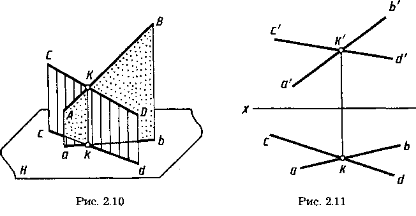
\includegraphics{img/241.png}\\
Пересекающиеся прямые -- если прямые пересекаются то их одноименные проекции персекаются между собой а проекции точек пересечения лежат на одной линии связи. В системе VH справедливо для всях прямых кроме профильных и обратное утверждение, если точки пересечения одноименных проекций прямых лежат на одной линии связи то прямые пересекаются.\\
\[
	\frac{b' m'}{a' m'} = \frac{b m}{a m}	
\]
\[
	\frac{c' m'}{a' m'} = \frac{cm}{am}	
\]
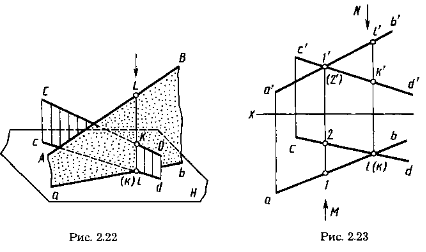
\includegraphics{img/242.png}\\
Параллельные прямые -- если прямые параллельны то их одноименные проекции параллельны между собой. Для прямых общего положения справедливо и обратное, если проекции прямых общего положения в системе двух плоскостей проекции параллельны то сами прямые также параллельны. Если одноименные проекции прямых параллельны одной из осей проекции то прямые параллельны при условии параллельности одноименных проекций на той плоскости проекций которой параллельны прямые.\\
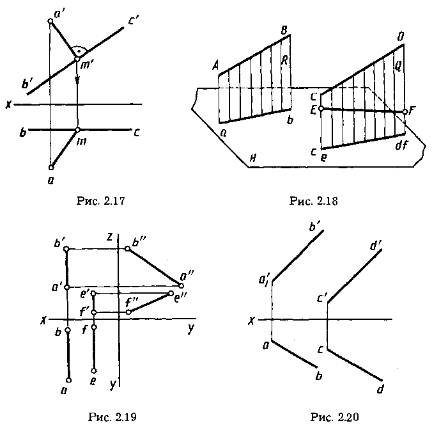
\includegraphics{img/243.png}\\
Скрещивающиеся прямые не имеют общих точек. Проекции скрещивающихся прямых пересекаются но точки пересечения проекций не лежат на одной линии связи.\\

\section{Глава. Плоскость}
\subsection{Положение плоскости относительно плоскостей проекции}

Плоскость можно задать разными способами:\\
-3мя точками, нележащими на одной прямой\\
-прямой и точкой, взятой вне этой прямой\\
-двумя пересекающимися прямыми\\
-двумя параллельными прямымы\\
-какая-либо плоская фигура\\

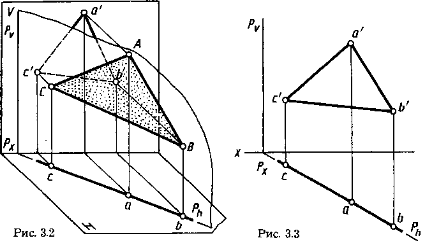
\includegraphics{img/311.png}\\
Положение плоскости по отношению к плоскотям проекции:\\
1)Плоскость не перпендикулярны плоскостям проекций(плоскость общего положения)\\
2)плоскость может быть перпендикулярна одной плоскости проекции(плоскости часного положения, проецирующие плоскости)\\
3)плоскость может быть перпендикулярна двум плоскостям проекции(плоскости часного положения, проецирующие плоскости)\\

След плоскости -- это линия пересечения плоскости с плоскостью проекции.\\

Для плоскости перпендикулярной плоскости H горизонтальный след PH распологается под углом к оси проекции X соответсвующе углу наклона этой плоскости к фронтальной плоскости проекции, а фронтальный след перпендикулярно оси X. Для плоскости перпендикулярной плоскости V фронтальный след распологается под углом к оси x соотвествующим углу наклона этой плоскости к плоскости H а горизонтальный след перпендикулярен оси X. На чертежах след перпендикулярный оси проекции не изображают.\\

Любая геометрическая фигура, лежащая в проецирующей плоскости, проецируется на соотвествующую плоскость проекции в прямую линию.\\
Плоскость перпендикулярна двум плоскостям проекции и параллельны третей.\\

\subsection{Прямая и точка в плоскости}
задачи:\\
1) Проведения прямой в плоскости\\
2) Построение в плоскости некоторой точки\\
3) Построение недостающей проекции точки\\
4) Проверка принадлежности точки плоскости\\

Если точка принадлежит плоскости то ее проекции лежат на проекции прямой принадлежащей плоскости.\\
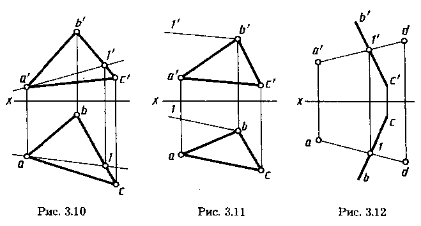
\includegraphics{img/321.png}\\


\subsection{Прямые особого положения плоскости-- главные линии плоскости}

Горизонтали(принадлежит плоскости и параллельна плоскости проекции H), фронтали(лежит в плоскости и параллельна фронтальной плоскости проекции), профильные(леж в плоскости и параллельна профильной плоскости проекции) прямые и линии наибольщего наклона.\\

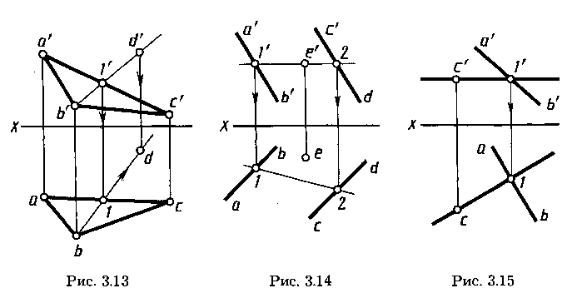
\includegraphics{img/331.png}\\
Линии наибольшего наклона  -- называют прямые лежащии в этой плоскости и перпендикулярные или к горизонталям или к ее фронталям или к ее профильным прямым\\

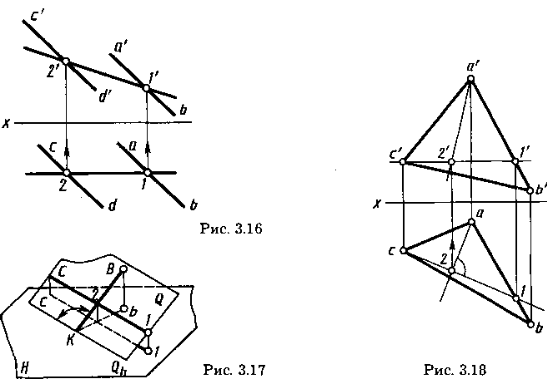
\includegraphics{img/332.png}\\


Угол между линией ската и ее горизонтальной проекцией является линейным углом между плоскостью, которой принадлежит линия ската, и плоскостью проекций Н\\

\section{ Глава. Взаимное положение прямой и линии в плоскости, двух плоскостей}

\subsection{Пересечение прямой линии с проецирующей плоскостью}

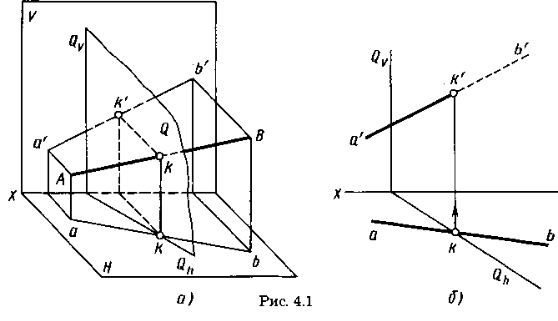
\includegraphics{img/411.png}\\


*для сложных чертежей анализ видимости мы не делаем*\\

Правила:\\
- Условно считают, что данная плоскость непрозрачна. Поэтому точки, линии, участки другой плоскости, расположенные между плоскостью проекций и данной плоскостью, невидимы для наблюдателя, между которым и плоскостью проекций находятся изображаемые объекты. Если линии, точки, участки другой плоскости находятся между данной плоскостью и наблюдателем, то они видимы и закрывают точки, линии, участки данной плоскости, лежащие на одних проецирующих прямых.\\

- Анализ видимости линий обычно проводят путем анализа видимости точек, как это сделано при анализе видимости конкурирующих точек на скрещивающихся прямых\\

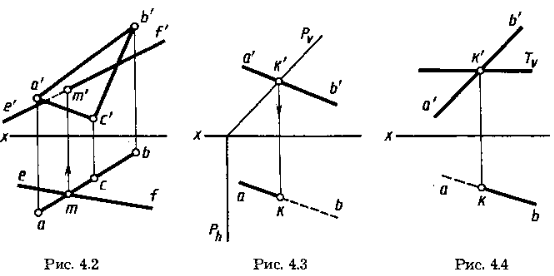
\includegraphics{img/412.png}\\


\subsection{Пересечение двух плоскостей}

*ДОСТАТОЧНО ПОСТРОИТЬ ОДНУ ТОЧКУ А ВТОРУЮ ТОЧКУ МОЖНО ПОЛУЧИТЬ ТАКИМ ЖЕ СПОСОБОМ*

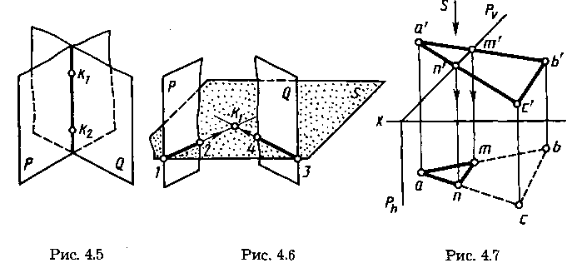
\includegraphics{img/421.png}\\

Для того чтобы найти точку принадлежащую двум плоскостям вводим вспомогательную плоскость строят линии пересечения вспомогательной плоскости с двумя заданными плоскостями и в пересечении построенных линий находят общую точку двух плоскостей. Для нахождения второй общей точки построение повторяют с помощью еще одной вспомогательной плоскости.\\

Частный случай построения линии пересечения двух плоскостей, когда одна из них проецирующая. В этом случае построение линии пересечения упрощается тем, что одна ее проекция совпадает с проекцией проецирующей плоскости на ту плоскость проекций, к которой она перпендикулярна.\\


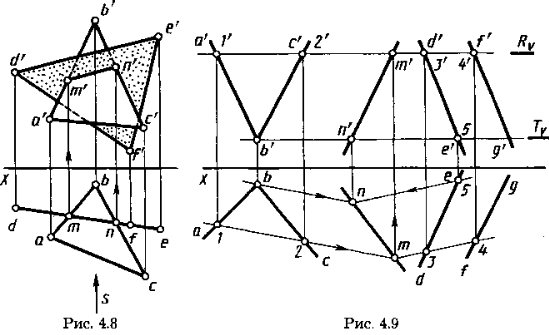
\includegraphics{img/422.png}\\
Построение линии пересечения плоскостей общего положения. На рисунке 4.9 приведено построение проекций т'п', тп линии пересечения двух плоскостей, одна из которых задана проекциями а'b', b'с’, ab, bс двух пересекающихся прямых, другая — проекциями d’e’, f'g', de, fg двух параллельных прямых.\\

Вспомогательные плоскости параллельны друг-другу.\\


\subsection{ Пересечение прямой линии общего положения с плоскостью общего положения}

Точку пересечения прямой с плоскостью общего положения строят в следующем порядке:\\
а)    через заданную прямую АВ проводят вспомогательную плоскость Т;\\
б)    строят линию пересечения 1—2 вспомогательной плоскости Т и заданной плоскости Q;\\
в)    в пересечении построенной линии 1—2 с заданной прямой АВ отмечают искомую точку К.\\

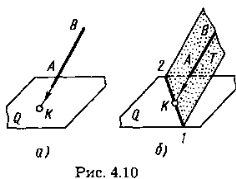
\includegraphics{img/431.png}\\

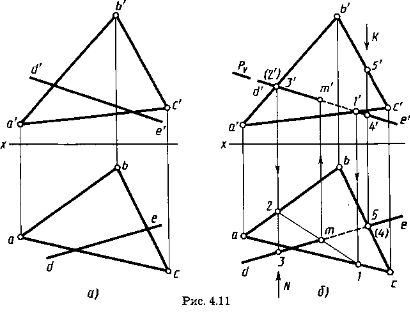
\includegraphics{img/432.png}

\subsection{ Построение взаимно-параллельных прямой и плоскости, двух плоскостей}
\subsubsection{Построение взаимно параллельных прямой линии и плоскости}

\quad \quad \quad \quad \quad \quad \quad 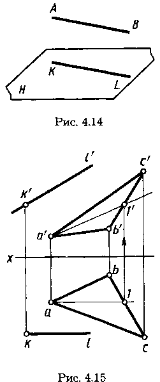
\includegraphics{img/441.png}\\

Для построения прямой, проходящей через заданную точку пространства параллельно заданной плоскости, достаточно провести прямую, параллельную любой прямой, принадлежащей плоскости.
При этом возможно бесчисленное множество решений. Дополнительные требования могут обусловить единственное решение.

Если необходимо проверить параллельна ли прямая заданной плосоксти нужно построить прямую параллельную заданной прямой в плоскости(если не существует -- то они не параллельны).

\subsubsection{Построение взаимно параллельных плокостей}

Если две пересекающиеся прямые, лежащие в одной плоскости, взаимно параллельны двум пересекающимся прямым лежащим в другой плоскости то плоскости параллельны.\\
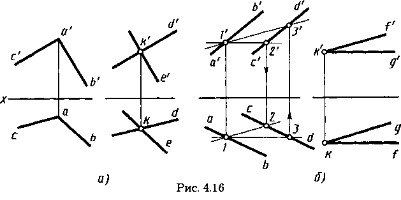
\includegraphics{img/442.png}\\

\subsection{Построение взаимно перпендикулярных прямой и плоскости}

\quad \quad \quad \quad \quad \quad \quad \quad 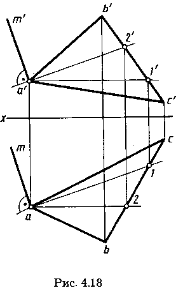
\includegraphics{img/451.png}\\
Если прямая перпендикулярна двум пересекающимся прямым, принадлежащим плоскости, то она перпендикулярна этой плоскости.\\

Чтобы построить две взаимно перпендикулярных плоскости необходимо построить перпендикуляр к одной из плоскостей а затем провести через одну из точек данного перпендикуляра  прямую, не принадлежащую исходной плоскости.

\subsection{Угол между прямой и плоскостью}
\quad \quad \quad \quad \quad \quad \quad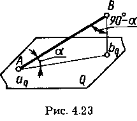
\includegraphics{img/461.png}\\
Угол между прямой и плоскостью определяется углом между этой прямой и ее проекцией на плоскости. Для решения этой задачи требуется:\\
1) найти точку пересечения прямой с плоскостью\\
2) провести из некоторой точки прямой перпендикуляр на плоскость.\\
3) определить точку пересечения перпендикуляра с плоскостью.\\
4) соединить эти точки линией\\\
5) определить угол между прямой и плоскостью\\
Ообычно достаточно построить только перпендикуляр. Задача определения угла между двумя прямыми расматривалась нами когда мы решали задачу определения угла наклона прямой к плоскости.

\section{Глава. Способы преоброзования чертежа}
\subsection{Общая характеристика способов преоброзования чертежа}

Многие задачи рашаются легко если линии и плоскии фигуры, образующие объект находятся в частном положении. Такого добится позволяет преоброзование чертежа, добится которого позволяют пару способов:\\
1) Переменной плоскостей проекции(в этом случае заданную систему плоскостей и проекций заменяют на новую так, чтобы исходные объекты не меняя своего положения в пространстве оказались в частном положении).\\
2) Способ вращения(в этом случае не измения плоскостей проекции исходные объекты поварачивают таким образом, чтобы они приняли частное положение).\\

\subsection{Способ перемены плоскостей проекции}
-- при этом способе преоброзовании чертежа положение точек, линий, плоских фигур, поверхностей в пространстве не изменяется, а система VH дополняется плоскостями, образующими с V или H или между собой систему двух взаимно перпендикулярных плоскостей, принемаемых за плоскости проекции.\\
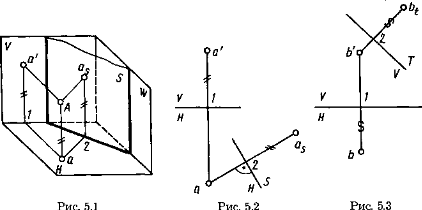
\includegraphics{img/521.png}\\

Можно проводить несколько раз.\\

4 основные задачи преобразования:\\
1) определение величины отрезка общего положения.\\
2) приведение плоской фигуры общего положения в проуцирующее положение.\\
3) Определение натурального вида плоской фигуры, расположенной в проецирующем положении.\\
4)Приведение отрезка прямой общего положения в проецирующее положение.
%Отредактировать изображения
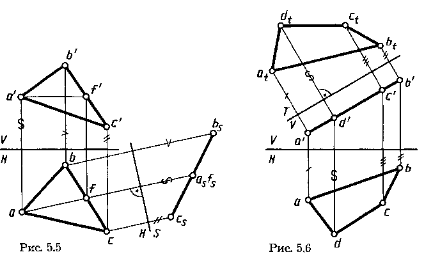
\includegraphics{img/522.png}\\
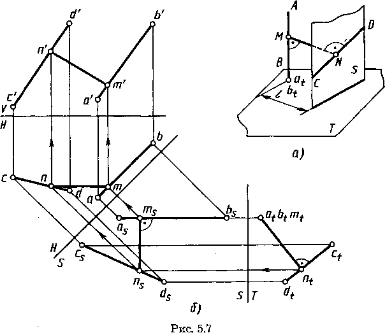
\includegraphics{img/523.png}\\
с помощью переменной плоскостей проекции можно определять растояние, это растояние представляет собой длинну общего перпенидкуляра,его длину удобно определять когда одна из скрещивающихся прямых находится в проецирующем положениию, таким образом мы вводим новую плоскость проекций такую,в которой одна из прямых находится в проецирующем положении, строим перпендикуляр ко второй прямой и определяем его длину.\\

\subsection{Способ вращения}

чтобы применить преобразование чертежа необходимо задать  несколько элементов:\\
1. ось вращения\\
2. плоскость вращения точки\\
3. центр вращения\\
4. радиус вращения(растояние от центра вращения до точки)\\
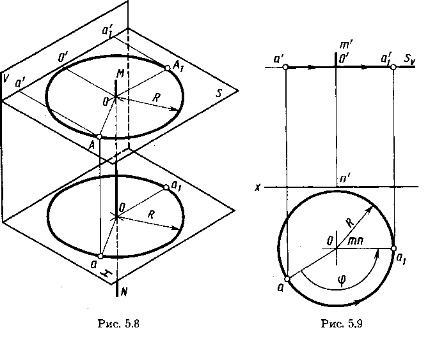
\includegraphics{img/531.png}\\

В качестве оси вращения обычно используют прямые, перпендикулярные или параллельные плоскостям проекций. Она может быть прямой общего положения но на практике не применяется.\\

Вращение точки A относительно MN, перпендикулярной относительно плоскости проекции.\\
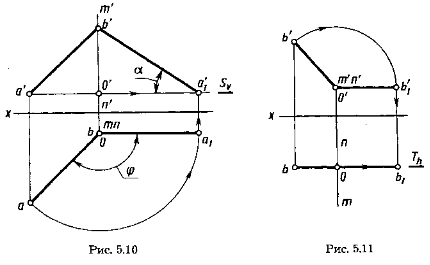
\includegraphics{img/532.png}\\

Вращение вокруг прямых параллельных плоскостям проекции\\
-- Натуральную велечину фигуры можно определить вращением вокруг оси параллельной плоскости проекции. В этом случае одним поворотом фигура приводится в плоскость параллельную плоскости проекции.\\

\end{document}